\documentclass[11pt]{amsart}
\usepackage{geometry}  % See geometry.pdf to learn the layout options.
\geometry{letterpaper} % ... or a4paper or a5paper or ... 
\usepackage{graphicx}
\usepackage{amssymb}
\usepackage{epstopdf}
\DeclareGraphicsRule{.tif}{png}{.png}{`convert #1 `dirname #1`/`basename #1 .tif`.png}

\title{Final Report}
\author{Juan Durazo \\ Arthur Mitrano \\ Brendan Horan}
\date{May, 2013}  

\begin{document}

\maketitle

\section{Introduction}
\subsection{Problem} \indent \\
The problem we are seeking to solve is 
\begin{equation*}
  Ax=b, \indent A  \in  \mathbb{R}, \indent b = b^{exact} + b^{noise}.
\end{equation*}
In the above equation, $b^{noise}$ is a white noise vector with unknown level 
$\delta_{noise}$. We investigate how noise enters the problem through $b$ and 
how it propagates into the core problem. Using this information, we can develop
a stopping criteria for hybrid methods that are based on the Golub-Kahan 
bidiagonalization(GKb) process. Additionally, we can estimate the original noise
level that was introduced into the problem with $b$.

\section{Golub-Kahan iterative bidiagonalization}
Given the initial vector $w_{0}$ and $s_{1} = b/\beta_{1}$, where 
$\beta_{1} = \|b\| \neq 0$, the Golub-Kahan iterative bidiagonalization is
discribed by
\begin{align*}
  \alpha_{j}w_{j} &= A^{T}s_{j} - \beta_{j}w_{j-1}, &\quad \|w_{j}\|=1,\\
  \beta_{j+1}s_{j+1} &= Aw_{j} - \alpha_{j}s_{j}, &\quad \|s_{j+1}\|=1
\end{align*}
until $\alpha_{j} = 0$ or $\beta_{j+1} = 0$, or we reach the dimensionality of
the problem. Letting $S_{k} = [s_{1},\ldots,s_{k}]$ and 
$W_{k}= [w_{1},\ldots,w_{k}]$ be the left and right bidiagonalization matrices,
then:
\begin{equation*}
  A^{T}S_{k} = W_{k}L_{k}^{T}, \quad AW_{k} = [S_{k},s_{k+1}]L_{k+},
\end{equation*}
where
\begin{equation*}
  L_{k} =
  \begin{bmatrix}
    \alpha_{1} & & & \\
    \beta_{2} & \alpha_{2} & & \\
    & \ddots & \ddots & \\
    & & \beta_{k} & \alpha_{k}
  \end{bmatrix}, \quad
  L_{k+} = 
  \begin{bmatrix}
    L_{k} \\
    \beta_{k+1}e_{k}^{T}
  \end{bmatrix}
\end{equation*}
Since this process leads to orthogonal matrices $S_{k}$ and $W_{k}$, we can
calculate the singular value decomposition of A as $A = S_{k}L_{k}W_{k}^{T}$
$= S_{k}U\Sigma V^{T}W_{k}^{T} = U_{k}\Sigma V_{k}^{T}$, with $U_{k}$ and 
$V_{k}$ orthogonal, since product of orthogonal matrices are orthogonal. This is
a stable way to calculate the SVD of $A$ \cite{svdRef}.

The GKIB applied on the problem $Ax = b$ is closely related to the
\emph{Lanczos tridiagonalization} of the matrix $AA^{T}$ with starting vector
$s_{1} = b/\beta_{1}$, $\beta_{1} = \|b\|$, yielding after $k$ steps:
\begin{equation} \label{eq:tridiag}
  AA^{T}S_{k} = S_{k}T_{k} + \alpha_{k}\beta_{k+1}s_{k+1}e_{k}^{T},
\end{equation}
with
\begin{equation*}
  T_{k} = L_{k}L_{k}^{T} = 
  \begin{bmatrix}
    \alpha_{1}^{2} & \alpha_{1}\beta_{2} & & \\
    \alpha_{1}\beta_{2} & \alpha_{2}^{2} + \beta_{2}^{2} & \ddots & \\
    & \ddots & \ddots & \alpha_{k-1}\beta_{k} \\
    & & \alpha_{k-1}\beta_{k} & \alpha_{k}^{2} + \beta_{k}^{2}
  \end{bmatrix}
\end{equation*}
The matrix $L_{k}$ is a Cholesky factor of the matrix $T_{k}$.
% Maybe we should add here information about the Ritz values or move this to a
% different section.

If we look for solutions of the original problem $Ax \approx b$ on the range of
$W_{k}$, i.~e.~, considering $x_{k} = W_{k}y_{k}$ as such solution, the residual
can be expressed as
\begin{align*}
  r_{k} = b - AW_{k}y_{k} &= S_{k+1}(\beta_{1}e_{1} - L_{k+}y_{k}) \\
  &= S_{k}(\beta_{1}e_{1} - L_{k}y_{k}) - 
  (\beta_{k+1}e_{k}^{T}y_{k})s_{k+1},
\end{align*}.
Using the orthogonality of $s_{k}$'s and the residual expression, we get two 
classes of subproblems:
\begin{enumerate}
  \item If we require that the residual $r_{k}$ to be orthogonal to $S_{k}$:
    \begin{equation*}
      L_{k}y_{k} = \beta_{1}e_{1}, \quad L_{k} \in \mathbb{R}^{k \times k},
    \end{equation*}
    which corresponds to the CGME(?) method.
  \item If we minimize the norm of the residual we get
    \begin{equation*}
      y_{k} = argmin_{y}\|L_{k+}y - \beta_{1}e_{1}\|
    \end{equation*}
    which corresponds to CGLS or LSQR method.
\end{enumerate}
For both kinds of subproblems the information used depends on the vector $b$ and
the bidiagonal matrix ($L_{k}$ or $L_{k+}$), this often refer as the core or
projected problem. The bidiagonalization concentrates the useful information of
the main problem on its bidiagonal block. In presence of noise, those
subproblems might be polluted by it. A better understanding on how this noise
propagates through the GKIB may aid on solving the ill-posed problem.

\section{Test problem: Shaw}
Most of the numerical experiments presented in this report are based on the 
problem \texttt{shaw(400)} from the Regularization Toolbox \cite{hansen}. $A$,
$b^{exact}$ and the exact solution $x$ are created by 
\texttt{[A, b\_exact, x] = shaw(400)}. Noise is added ($b^{noise}$) using the
Matlab \texttt{rand(400,1)}, which is scaled such that
\begin{equation*}
  \delta_{\text{noise}} = \frac{\|b^{\text{noise}}\|}{\|b^{\text{exact}}\|}.
\end{equation*}
We used $\delta_{\text{noise}} = 10^{-14}, 10^{-8}, 10^{-4}, 10^{-2}$ as noise level.
The shaw problem satisfy the \emph{discrete Picard condition} on average 
(without added noise). On figure \ref{fig:picard} we see that the Picard 
condition is drastically violated due to the complete dominance of the noise in
the projections of $b$ onto the left singular vectors $u_{j}$ of $A$.

\begin{figure}[htb] \label{fig:picard}
  \begin{center}
    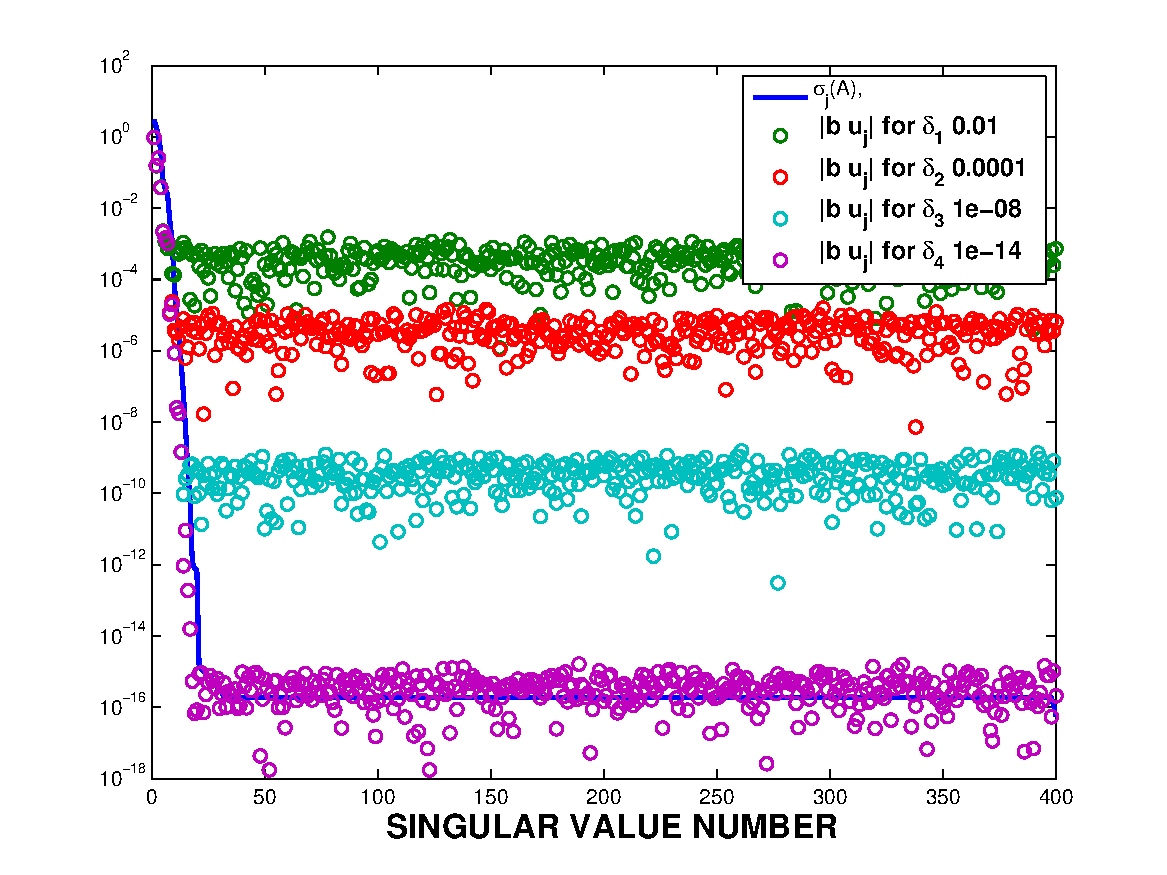
\includegraphics[width=.55\linewidth]{../presentation/figures/picard}
  \end{center}
\caption{Singular values $\sigma_{j}$ and the absolute value of the
projections of the noisy right-hand side $b$ on the left singular vectors 
$u_{j}$ of $A$. $\delta_{\text{noise}} = 10^{-14}, 10^{-8}, 10^{-4}$.}
\end{figure}

\section{Analyzing the spectral coefficients of $s_{k}$}
Now we focus our attention on studying and interpreting the spectral 
coefficients of the vectors $s_{k}$. This will give the information on how the
noise spreads on the problem solution.

The singular vectors $u_{k}$ increase in frequency as $k$ increases, as 
see in figure \ref{fig:singularVectors}.
In figure \ref{fig:spectralCoeffs} we see that as $k$
is increased the spectral coefficients associated with the lower frequency 
singular vectors decay and the ones associated with the high frequencies rise 
until they are comparable. This behavior is consider to reveal the noise.
\begin{figure}[b] \label{fig:singularVectors}
  \begin{center}
    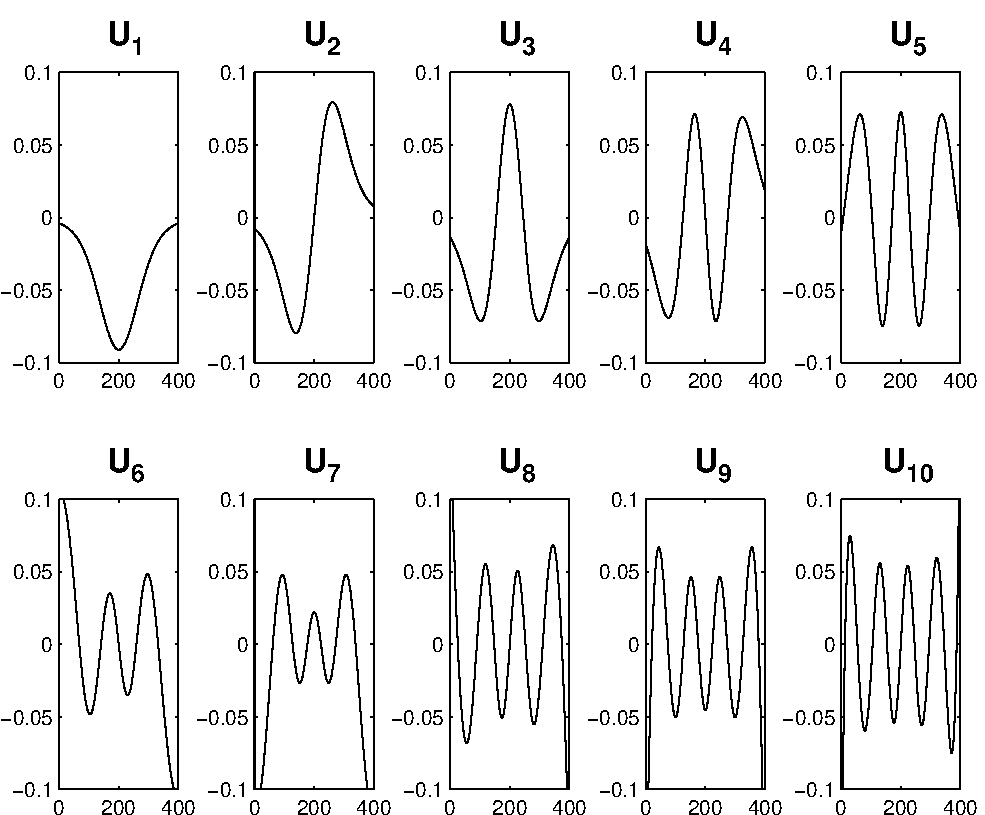
\includegraphics[width=0.55\linewidth]{figures/run1/sing_vecs}
  \end{center}
\caption{Note that the frequency of the singular vector increase with $k$.}
\end{figure}
\begin{figure}[htb] \label{fig:spectralCoeffs}
  \begin{center}
    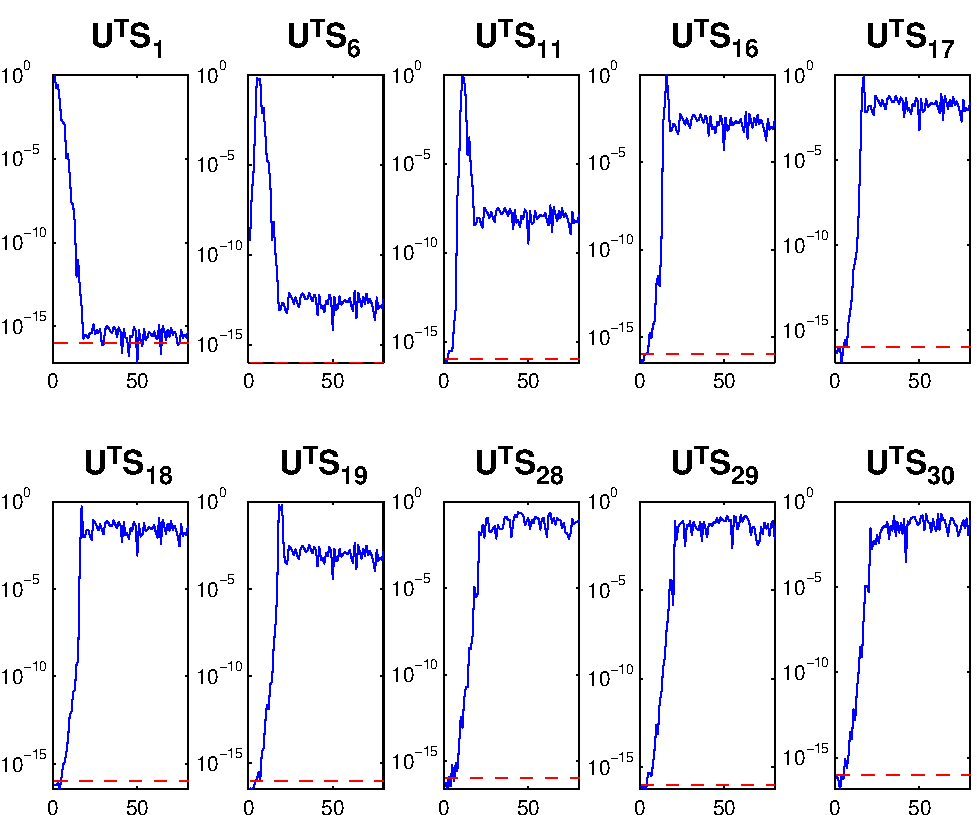
\includegraphics[width=0.55\linewidth]{figures/run1/spec_sk}
  \end{center}
\caption{Plot of the first 80 spectral coefficients on the direction of the left
singular vectors of $A$. As $k$ increases the lower frequencies get filtered out
and the high frequencies become comparable. $\delta_{\text{noise}} = 10^{-14}$}
\end{figure}

To better see what is happening we can use the singular value decomposition of
$A$ and the Lanczos tridiagonalization \eqref{eq:tridiag} of $AA^{T}$ to deduce
\begin{equation} \label{eq:spectralCoeffs}
  \Sigma^{2}(U^{T}S_{k}) = (U^{T}S_{k})(L_{k}L_{k}^{T}) + 
  \alpha_{k}\beta_{k+1}(U^{T}s_{k+1})e_{k}^{T}.
\end{equation}
Setting $k = 1$ we can see how the noise spreads from $s_{1}$ to $s_{2}$,
looking to the last column of \eqref{eq:spectralCoeffs} we get:
\begin{equation*}
  \alpha_{1}\beta_{2}(U^{T}s_{2}) = (\Sigma^{2} - \alpha_{1}^{2}I)U^{T}s_{1}.
\end{equation*}
So the spectral coefficients of $s_{2}$ are multiplied by
\begin{equation*}
  \frac{\sigma_{k}}{\alpha_{1}\beta_{2}} - \frac{\alpha_{1}}{\beta_{2}},
\end{equation*}
where the constant $\alpha_{1}/\beta_{2}$ is likely larger than 1. Hence, for 
$k$ small we are multiplying by smaller number, and for large $k$ values the
singular values $\sigma_{k}$ are negligible, which makes the spectral
coefficients associated amplified ($\alpha_{1}/\beta_{2}$) see section 3.1 of 
\cite{bidiagonalization} and figure \ref{fig:rhok}.

For the general case, we can rewrite equation \eqref{eq:spectralCoeffs} as
\begin{equation*}
  U^{T}s_{k+1} = \phi_{k}(\Sigma^{2})U^{T}s_{1}
\end{equation*}
where $\varphi_{k}(\lambda)$ is the Lanczos polynomial with roots 
$(\theta_{k}^{(k)})^{2}$, $l = 1,\ldots,k$, which are called \emph{Ritz values}.
The first singular values squared of $A$, $\sigma_{1}^{2}$, $\sigma_{2}^{2}$, 
\ldots closely approximates the large Ritz values 
$\left(\theta_{k}^{(k)}\right)^{2}$, $\left(\theta_{k-1}^{(k)}\right)^{2}$, 
\ldots. Moreover, the constant term
\begin{equation*}
  \phi_{k}(0) = \prod_{j=1}^{k}\frac{\alpha_{j}}{\beta_{j+1}} = \rho_{k}^{-1}.
\end{equation*}
In \cite{bidiagonalization}, one can find further details and references on how 
to deduce and confirm numerically those statements. 

Since the first singular values are close to the roots of
$\varphi_{k}(\lambda)$, the coefficients associated with low frequencies will be
filtered out. However, due to $rho_{k}$ getting small as $k$ increases (figure
\ref{fig:rhok}) and the singular values converging to zero, we have an
relative amplification of the high frequency noise components present on 
$s_{1}$.
\begin{figure}[htb] \label{fig:rhok}
  \begin{center}
    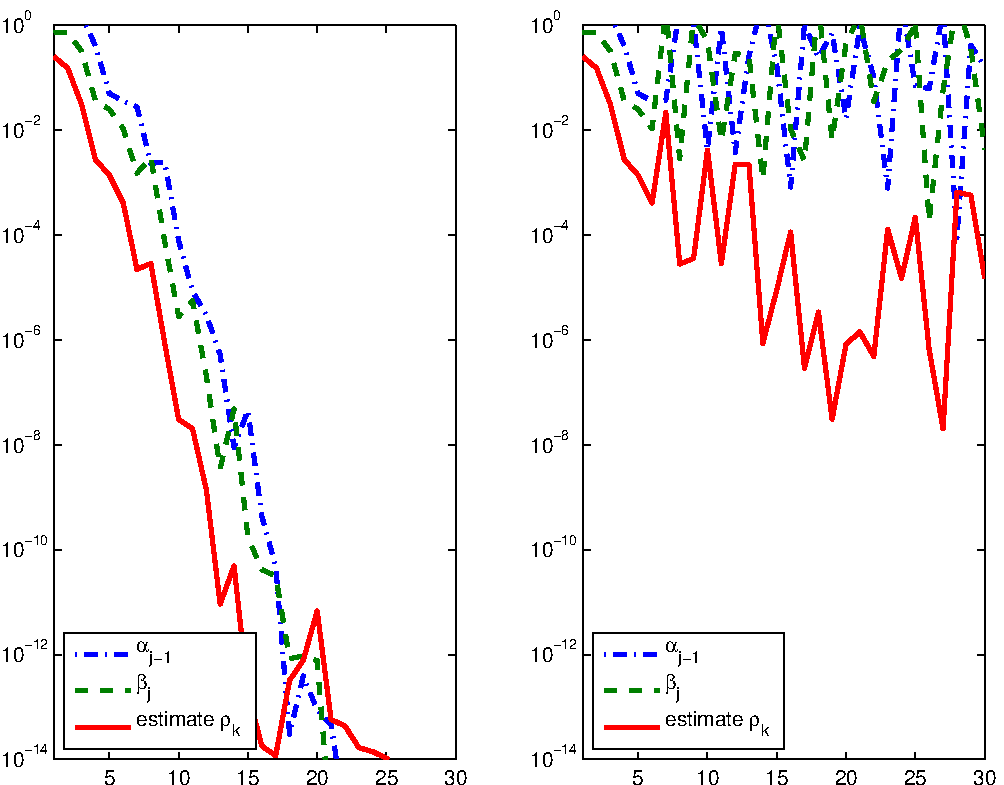
\includegraphics[width=0.55\linewidth]{figures/run1/alpha_beta_est}
  \end{center}
\caption{The left plot uses double reorthogonalization and the right one does
not. The reader can find information of noise propagation when orthogonality of
the bidiagonal vectors is lost in \cite{bidiagonalization} section 5.}
\end{figure}

Synthesizing, $s_{2},s_{3},\ldots$ will have dominant components in the
direction of the left singular vectors $u_{2},u_{3},\ldots$, respectively, with
the high frequency noise components gradually increasing. At some point
$k = k_{\text{noise}}$, the vector $s_{k_{\text{noise}} + 1}$ will have
comparable components on all the subspaces associated with the singular values
$\sigma_{k_{noise} + 1}, \sigma_{k_{noise} + 1}, \ldots$, and this will 
\emph{reveal} the noise. We can see this behavior on figure 
\ref{fig:spectralCoeffs}, which indicates that $k_{\text{noise}} = 17$. In
figure \ref{fig:snSpace} we display an automate criteria to reveal the value of
$k_{\text{noise}}$. We observe that as $k$ increases the $s_{k+1}$ gets closer
to the noise subspace (rotates counterclockwise), but the vector $s_{19}$ moves
clockwise, approaching the signal space. This indicates that the noise is
revealed in $s_{18}$, which justifies the reveling noise iteration to be 
$k_{\text{noise}} = 17$.
\begin{figure}[htb] \label{fig:snSpace}
  \begin{center}
    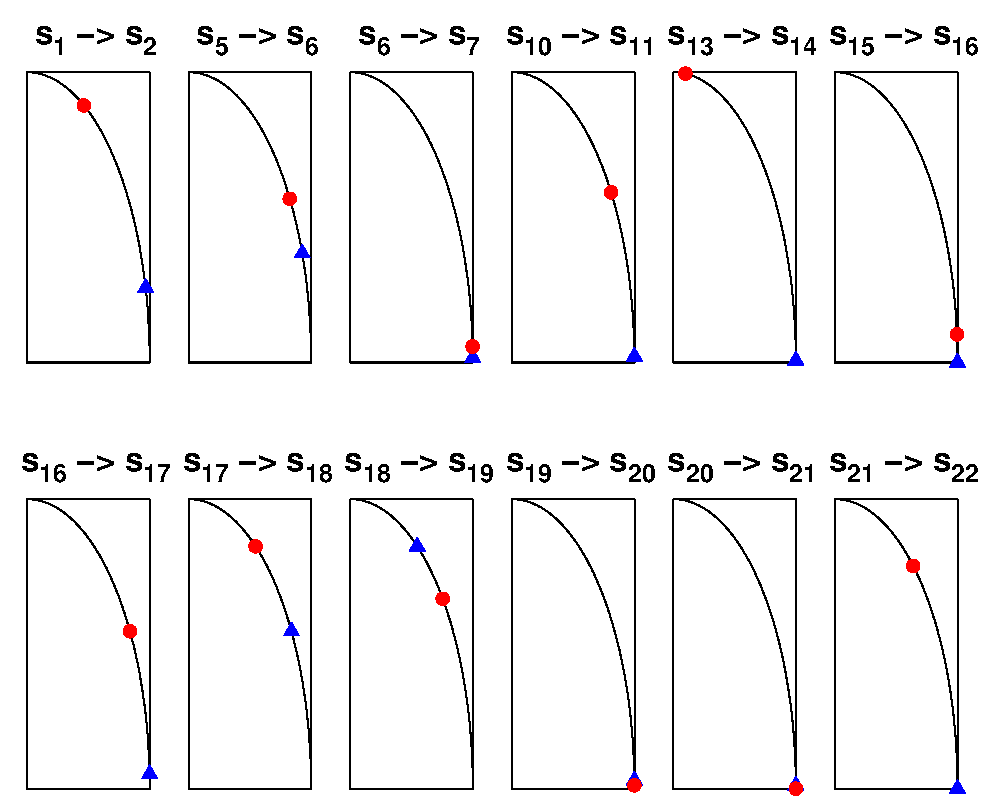
\includegraphics[width=0.55\linewidth]{figures/run1/signal_noise_space}
  \end{center}
\caption{The $span\left\{u_{1},\ldots,u_{k+1}\right\}$ is the signal subspace 
(\emph{horizontal axis}) and $span\left\{u_{k+2},\ldots,u_{n}\right\}$ is the
noise subspace (\emph{vertical axis}). The abscissa and ordinate of the vector 
$s_{k}$ are given by its projection on the signal and noise subspaces, 
respectively. ($\triangle$): $s_{k}$ and ($\circ$): $s_{k+1}$.}
\end{figure}

\section{Behavior of $s_{k}^{\text{exact}}$ and $s_{k}^{\text{noise}}$}
To further illustrate the noise amplification we look to $s_{k}^{exact}$ and 
$s_{k}^{noise}$. Let $s_{1} = s_{1}^{exact} + s_{1}^{noise}$ and define the
$s_{k}^{exact}$ and $s_{k}^{noise}$ by
\begin{align*}
  \beta_{k+1}s_{k+1}^{exact} &= Aw_{k} - \alpha_{k}s_{k}^{exact}, \\
  \beta_{k+1}s_{k+1}^{noise} &= -\alpha_{k}s_{k}^{noise}, \\
  s_{k+1} &= s_{k+1}^{exact} + s_{k+1}^{exact}, \quad 
  \beta_{k+1}s_{k+1} = Aw_{k} - \alpha_{k}s_{k}.
\end{align*}
Those vector aren't the true exact and noise data, but they give good 
approximations to their euclidean norm. For more details see 
\cite{bidiagonalization}.

\section{Cumulative periodogram}
The normalized cumulative periodogram (NCP) can be used to determine how 
``white-noise like'' each $s_k$ is. Given a sequence of $s_k$ we can compute the
vectors
$$c_k = |dft(s_k)|^2, \indent z_k = \frac{\sum_{i=1}^k c_i}{ \sum_{i=1}^q c_i}, \indent j=1,\cdots, q$$ 
The test is to see if any of the $z_k$ vectors are to a straight increasing diagonal line. There are two 
ways to measure how close the $z_k$ vectors are to this diagonal line. We can measure the 
absolute value of the deviation of each vector from the "white noise" diagonal line or we can keep
count of the number of indices that lie outside the Kolmogorov-Smirnov test at a certain confidence 
level. 

\section{Results}

\subsection{Finding $\bf k_{noise}$ using GKIB} \indent \\
	Recall that we can find the iteration $k_{noise}$ in which the noise is revealed automatically
	using the noise-signal space computations and also by looking at plots of the $s_k$ vectors.
	First, we will use the latter approach to present to see for what iteration, the noise {\it begins}
    to become visible.

	We first consider the case when $\delta_{noise}=10^{-14}$ and then consider the cases
	where $\delta_{noise} = 10^{-8},10^{-4},10^{-2}$:


	%%%%%%%%%%%%%%%%%%%%%%%%%%%%%%%%%%%%%%%%%%%%%%
	\vspace{5mm}
	\begin{minipage}[t]{0.5\textwidth}
	
		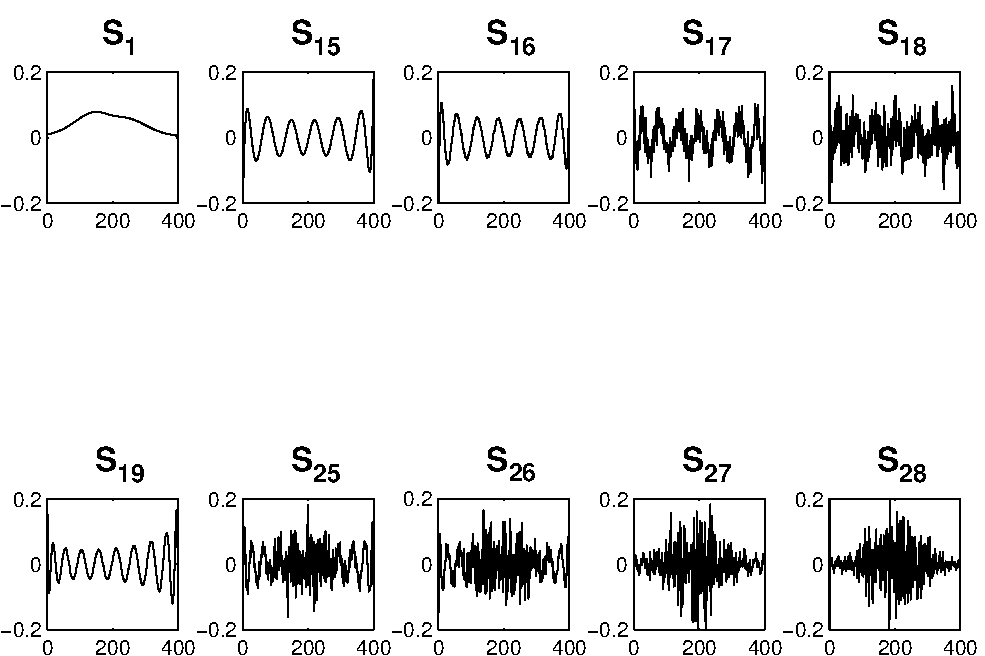
\includegraphics[width=.95\linewidth]{figures/run1/sk_plots} 
   
	\end{minipage}
	\begin{minipage}[t]{0.5\textwidth}
	
		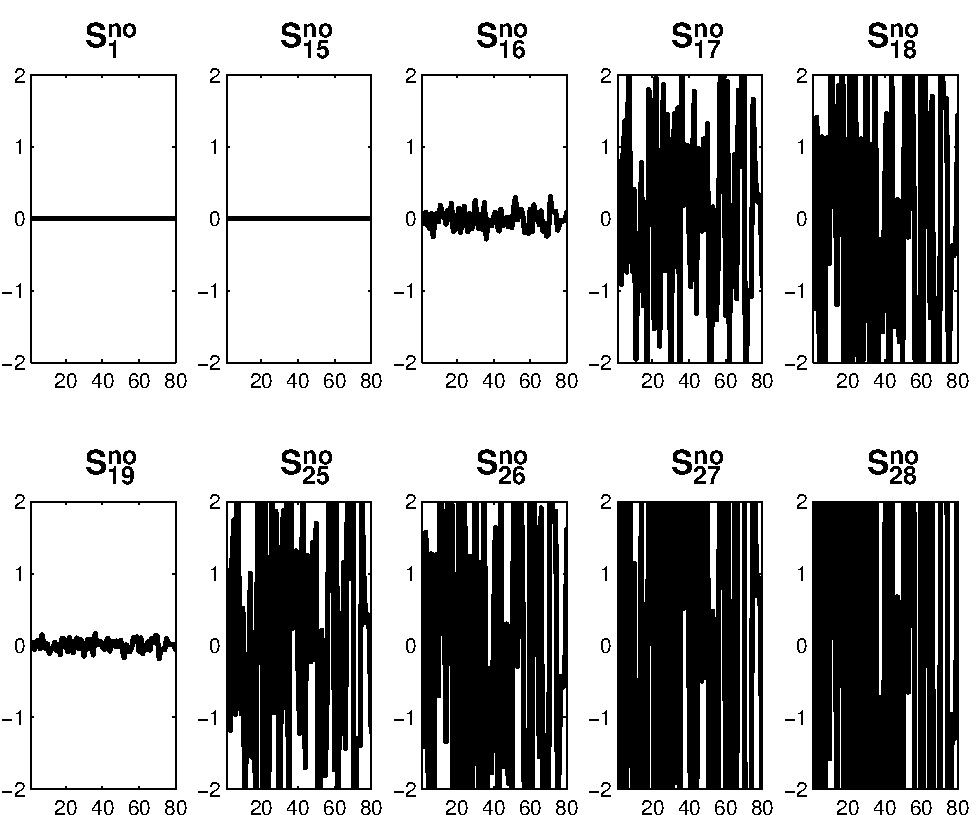
\includegraphics[width=.75\linewidth]{figures/run1/noise_parts} 
   
	\end{minipage}
	\begin{center}
		FIGURE: 
		The noise becomes visible at $s_{17}$, so $k_{noise} = 17$.
	\end{center} 
	\vspace{5mm}
	%%%%%%%%%%%%%%%%%%%%%%%%%%%%%%%%%%%%%%%%%%%%%%

	
	
	%%%%%%%%%%%%%%%%%%%%%%%%%%%%%%%%%%%%%%%%%%%%%%
	\vspace{5mm}
	\begin{minipage}[t]{0.5\textwidth}
	
		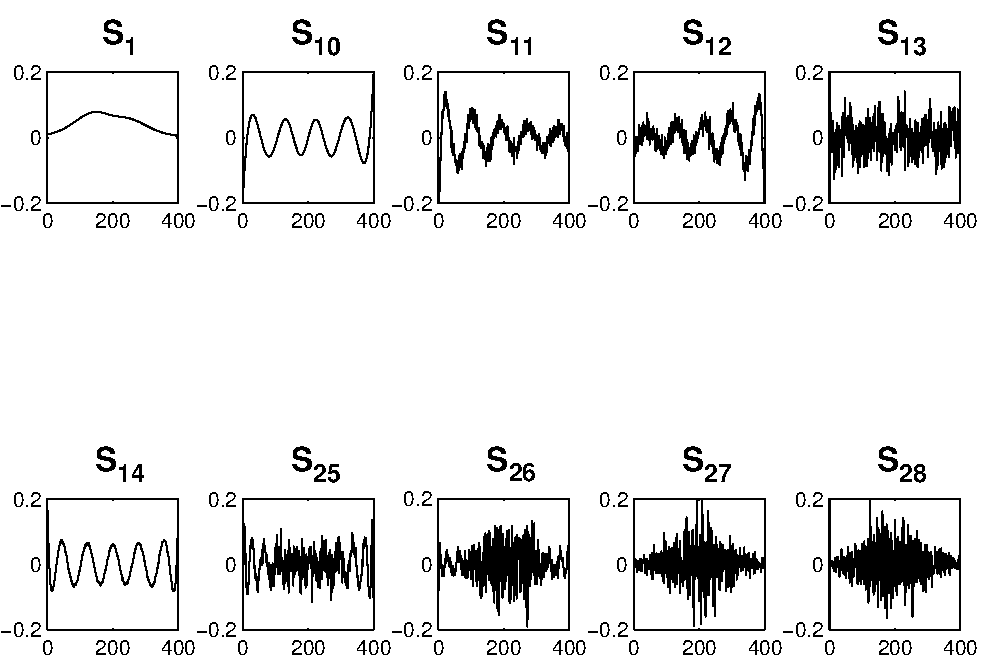
\includegraphics[width=.95\linewidth]{figures/run2/sk_plots} 
   
	\end{minipage}
	\begin{minipage}[t]{0.5\textwidth}
	
		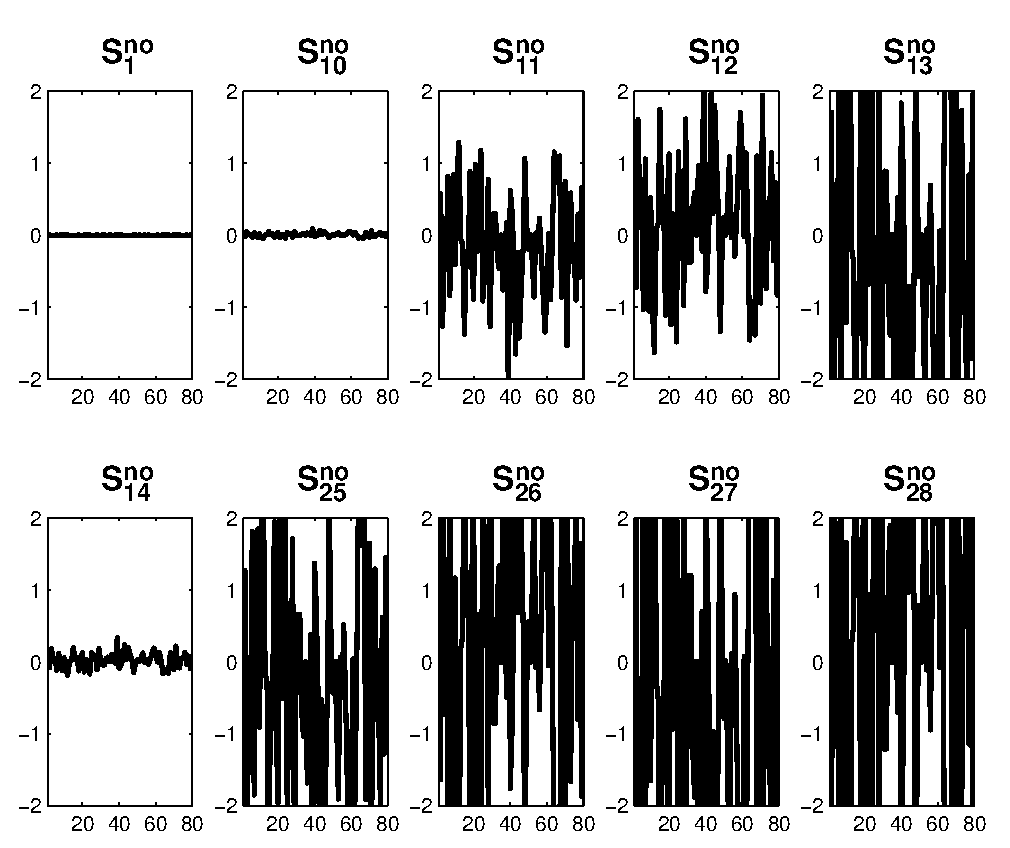
\includegraphics[width=.75\linewidth]{figures/run2/noise_parts} 
   
	\end{minipage}
	\begin{center}
		FIGURE: 
		Noise starts to become visible at $s_{11}$ for $\delta_{noise}=11$
	\end{center} 
	\vspace{5mm}
	%%%%%%%%%%%%%%%%%%%%%%%%%%%%%%%%%%%%%%%%%%%%%%
	
	%%%%%%%%%%%%%%%%%%%%%%%%%%%%%%%%%%%%%%%%%%%%%%
	\vspace{5mm}
	\begin{minipage}[t]{0.5\textwidth}
	
		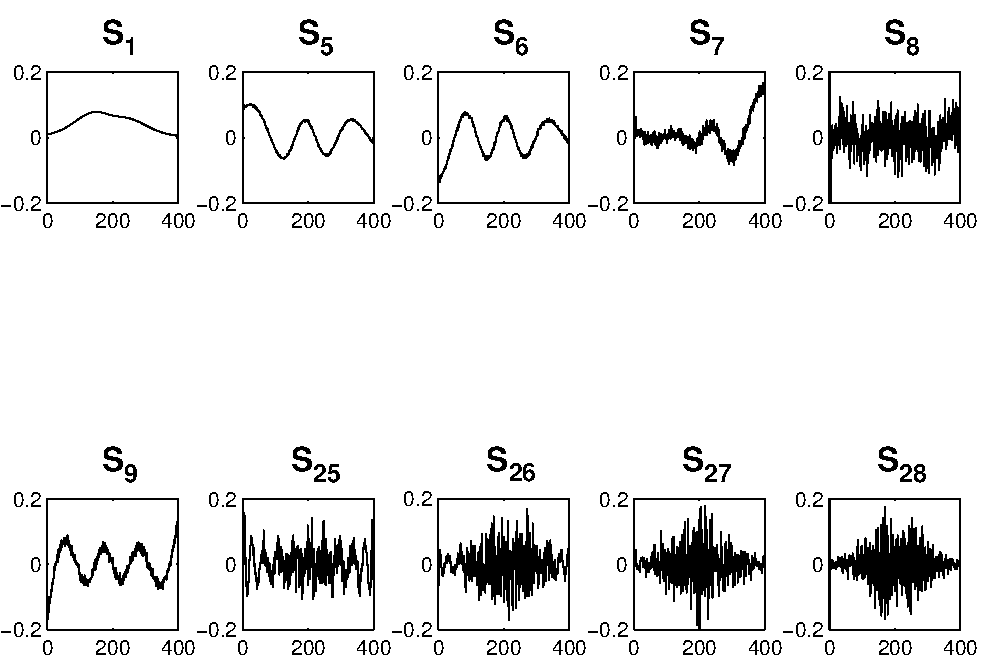
\includegraphics[width=.95\linewidth]{figures/run3/sk_plots} 
   
	\end{minipage}
	\begin{minipage}[t]{0.5\textwidth}
	
		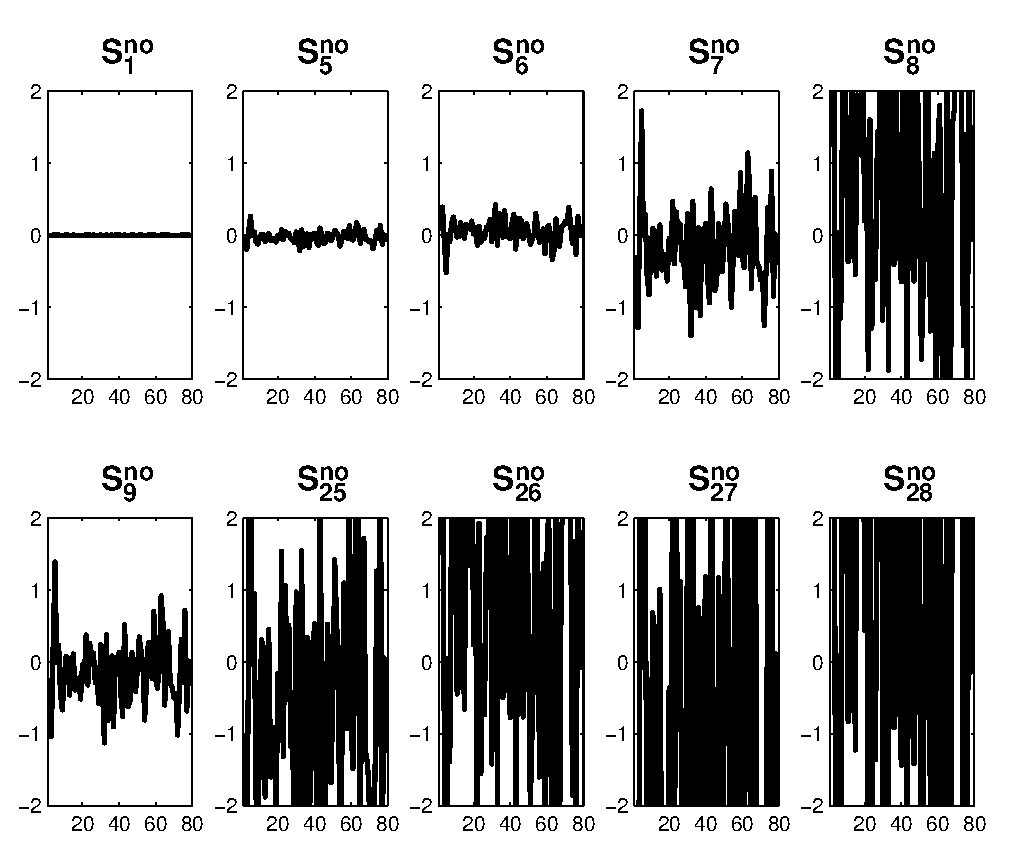
\includegraphics[width=.75\linewidth]{figures/run3/noise_parts} 
   
	\end{minipage}
	\begin{center}
		FIGURE: 
		Noise starts to become visible at the $s_{7}$ plot for $\delta_{noise}=7$
	\end{center} 
	\vspace{10mm}
	%%%%%%%%%%%%%%%%%%%%%%%%%%%%%%%%%%%%%%%%%%%%%%
	
	%%%%%%%%%%%%%%%%%%%%%%%%%%%%%%%%%%%%%%%%%%%%%%
	\vspace{10mm}
	\begin{minipage}[t]{0.5\textwidth}
	
		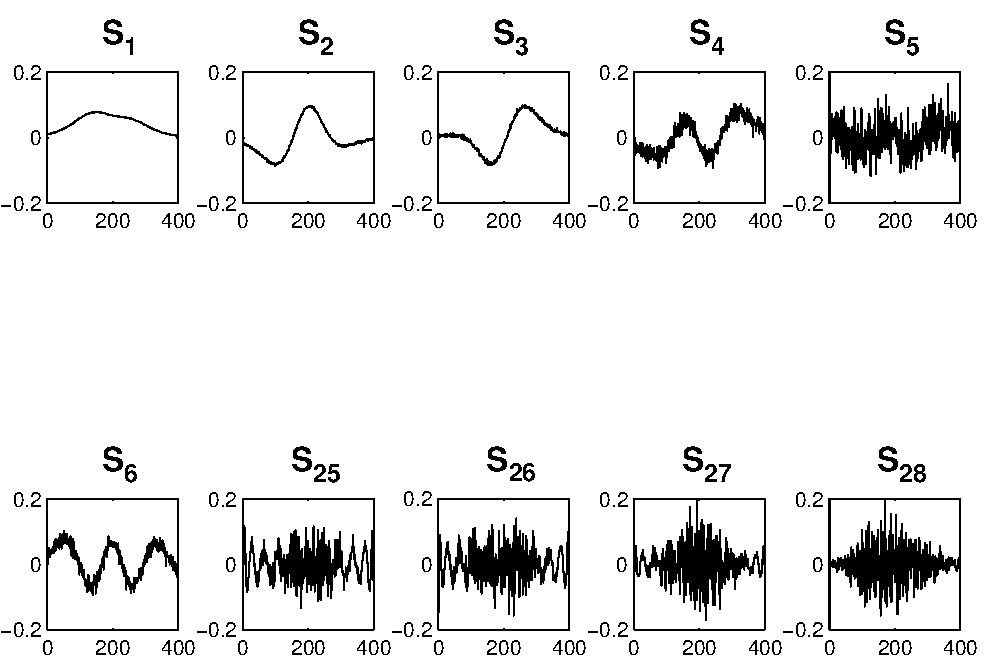
\includegraphics[width=.95\linewidth]{figures/run4/sk_plots} 
   
	\end{minipage}
	\begin{minipage}[t]{0.5\textwidth}
	
		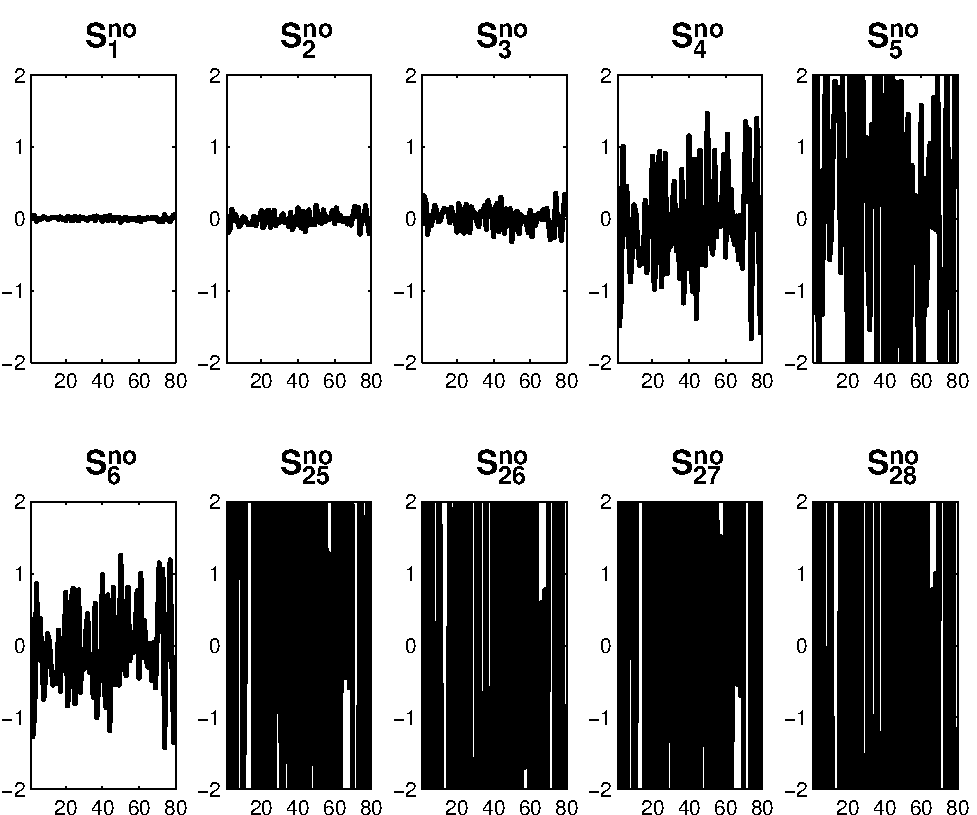
\includegraphics[width=.75\linewidth]{figures/run4/noise_parts} 
   
	\end{minipage}
	\begin{center}
		FIGURE: 
		Noise starts to become visible at the $s_{4}$ plot for $\delta_{noise}=4$	\end{center} 
	\vspace{10mm}
	%%%%%%%%%%%%%%%%%%%%%%%%%%%%%%%%%%%%%%%%%%%%%%
	
	
	As we can see in the above plots, for larger values of $\delta_{noise}$, the
	noise is revealed at earlier iterations. We also see that once the noise enters
	the $s_k$ vectors for the first time, the plots of $s_k$(left column) appear to have 
	reduced amount of noise in the immediately following iteration but this 
	noise then goes on to increase as $k$ increases. This observation can also be seen on the
	plots of $s_{k}^{no}$(right column).
	
We can automate the approximation of using the signal-noise space like in figure \ref{fig:snSpace}.
We can compute the iteration for when moving from the circle to the triangle is not a clockwise
rotation. This amounts to calculating the iteration where the horizontal coordinate of the circle is greater
than the horizontal coordinate of the triangle. It should be noted that sometimes coordinate of the 
circle is greater than the horizontal coordinate of the triangle, but only by about a small  amount of 
order $10^{-4}$ as in the 3rd plot in \ref{fig:snSpace}.
However this happens way before the noise revealing iterations found above visually . We therefore
ensure that coordinate of the circle is greater than the horizontal coordinate of the triangle by at least 0.1. 
Under this convention, we can find $k_{noise}$ values that are found visually above.

The step $k$ in which this happens corresponds to noise being projected out of the vector $s_k$,
which means that the noise is revealed in $s_{k-1}$. Therefore the noise revealing iteration 
is $s_{k-2}$. The table below contains the values of $k_{noise}$ that are found for the different 
values of $\delta_{noise}$.

\begin{center}
    \begin{tabular}{l||c|c|c|c}
      \multicolumn{1}{l||}{problem} & \multicolumn{4}{l}{\texttt{shaw(400)}} \\
      \hline \hline 
      $\delta_{noise}$ & $10^{-14}$ & $10^{-8}$ & $10^{-4}$ & $10^{-2}$ \\
      \hline
      $k_{noise}$ (GKIB) & $17$ & $11$ & $7$ & $4$ \\
          \end{tabular}
  \end{center}

\subsection{Finding $\bf k_{noise}$ using NCP} \indent \\
First we present the plot that we discussed during the presentation. This is the case where
$\delta_{noise} = 10^{-14}$  and the $\delta_{KS}=1.35$. Here, $\delta_{KS}$ is half of the
width of the Kolmogorov-Smirnov($KS$) test band. The corresponding cumulative periodogram is given below. 
On the left is the periodogram of the vectors $s_k$. On the right is their total deviation from 
the diagonal "white noise" diagonal line in blue and the percentage of indices lying outside of the KS test band.



%%%%%%%%%%%%%%%%%%%%%%%%%%%%%%%%%%%%%%%%%%%%%%
	\vspace{5mm}
	\begin{minipage}[t]{0.5\textwidth}
	
		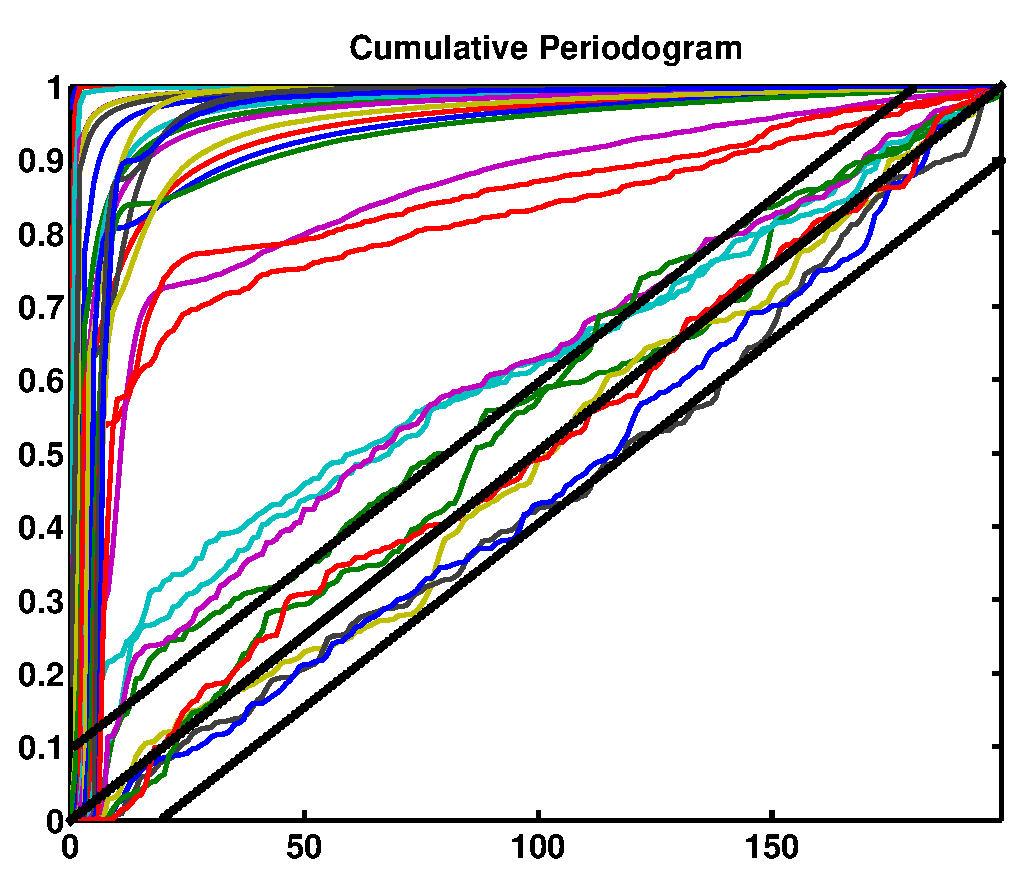
\includegraphics[width=.95\linewidth]{../presentation/figures/run1/cum_per} 
   
	\end{minipage}
	\begin{minipage}[t]{0.5\textwidth}
	
		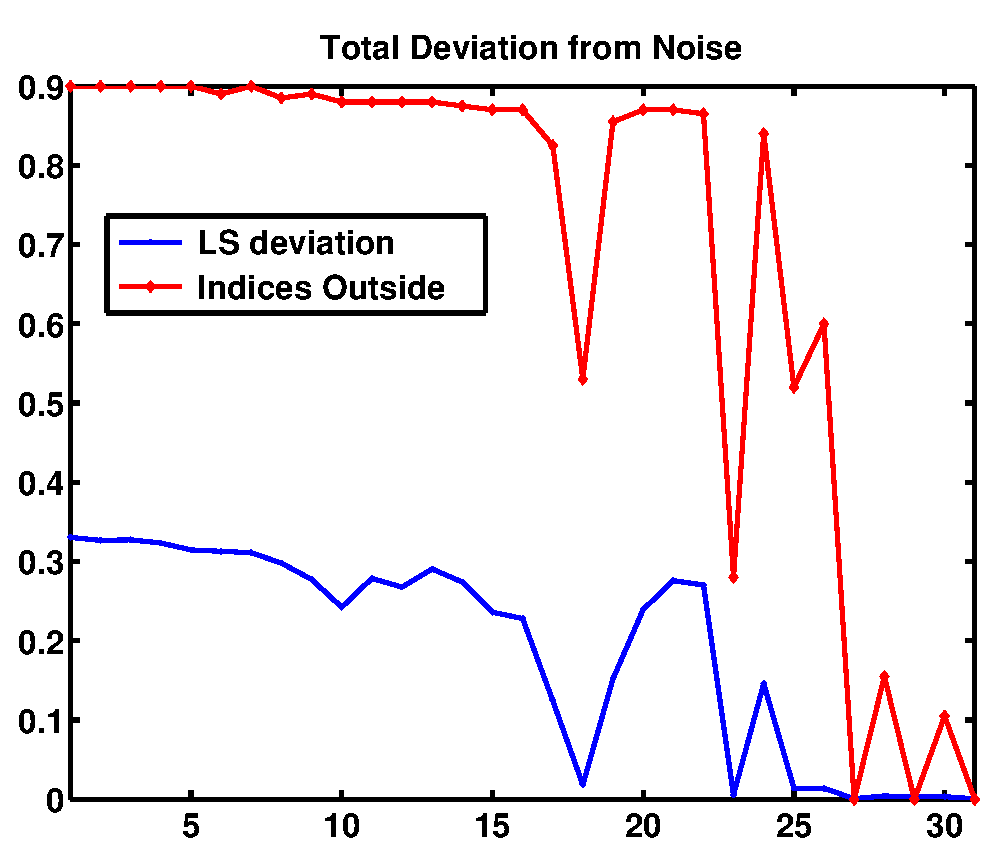
\includegraphics[width=.95\linewidth]{../presentation/figures/run1/total_deviation} 
   
	\end{minipage}
    \vspace{5mm}
	%%%%%%%%%%%%%%%%%%%%%%%%%%%%%%%%%%%%%%%%%%%%%%


As discussed in the presentation and can be see on the total deviation plot above, NCP
is determining that $k_{noise} = 27$. This value is in disagreement with the value determined
using KGIB value of 17. Looking again at the total deviation plot, we can see that at iteration 17,
there is a significant dip in total deviation and then it goes on to increase dramatically and then 
decrease again as it approaches iteration number 27. This is to be expected given the
behavior of the $s_k$ vectors that was discussed above. We saw that at iteration $k={17}$, 
there was an increase in visible noise. This corresponds to $S_{17}$ being closer to white noise
and hence we get the dip in the total deviation as well as the number of indices outside the 
KS band.  
Also recall that immediately after iteration
$k=17$, there was a drop in visible noise. This corresponds to these $s_k$ vectors being less
white noise like and this is reflected in the increase in total deviation and number of indices outside 
the KS band in the plot above. 
Finally, recall that after this decrease in visible white noise, we start to see more and more white 
noise in the $s_k$ vectors. This corresponds to the mostly decreasing total deviation
part of the plot above. 

Also from this plot, we can see that if NCP does not consider the first main dip to be white noise,
it won't happen again until after the fall and rise of white noise of the vectors $s_k$.

This suggests that our criteria of what we call white noise may be too strict. If we widen our KS band
a bit we may be able to have NCP agree with KGB as to which iteration is the noise revealing iteration.
This corresponds to increasing the $\delta_{KS}$ value, where $\delta_{KS}$ is half of the width
of the KS band. After some experimentation we found that in order to get 
$k_{noise}$ from the first dip, the value of $\delta_{KS}$ must be at about 8.15.
We are not sure if making such modifications are allowed to be made with this test however.
Using $\delta_{KS}=8.15$ and $\delta_{noise}=10^{-14}$, we get the plot below:

%%%%%%%%%%%%%%%%%%%%%%%%%%%%%%%%%%%%%%%%%%%%%%
	\vspace{5mm}
	\begin{minipage}[t]{0.5\textwidth}
	
		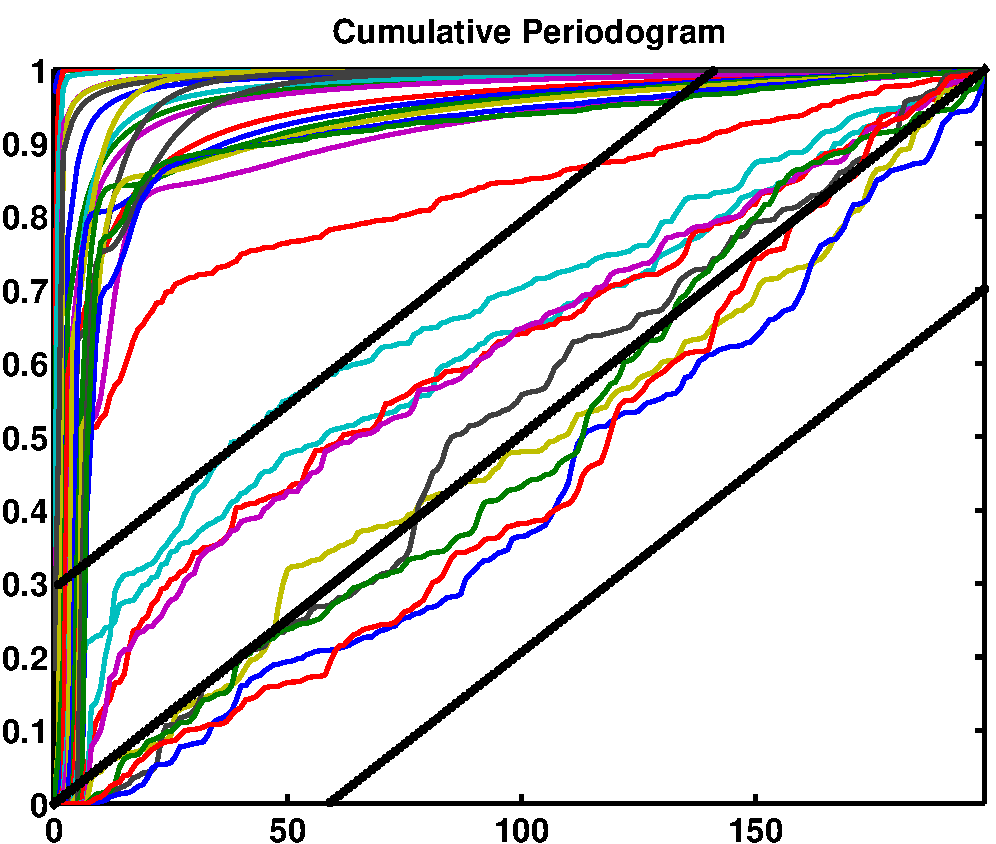
\includegraphics[width=.95\linewidth]{figures/run1/cum_per} 
   
	\end{minipage}
	\begin{minipage}[t]{0.5\textwidth}
	
		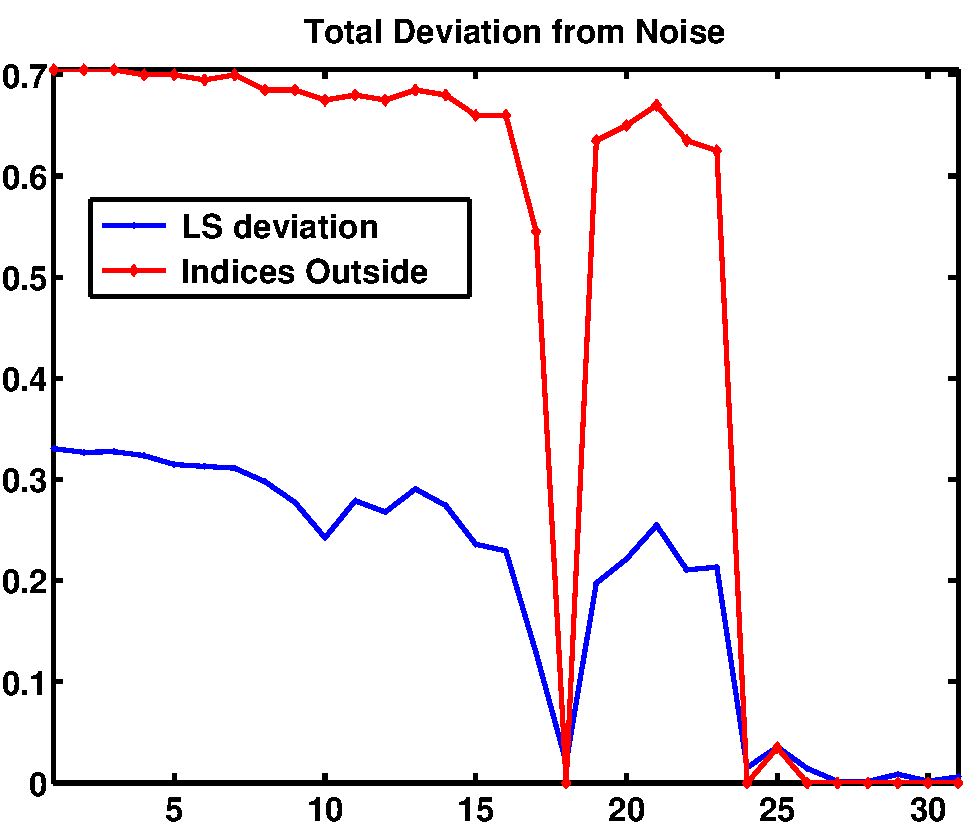
\includegraphics[width=.95\linewidth]{figures/run1/total_deviation} 
  
	\end{minipage}
{\centering $\delta_{noise}=10^{-14}$}
%%%%%%%%%%%%%%%%%%%%%%%%%%%%%%%%%%%%%%%%%%%%%%

Note that we want to get the iteration $k$ where noise is begins to reveal and not 
necessarily when the vector $s_k$ is dominated by white noise. Hence in determining
$k_{noise}$ with NCP, we find first iteration that is dominated by white noise, or 
in other words its corresponding $z_k$ vector is within the KS band, and we take 
$k_{noise}$ to be the previous iteration. Presumably, this is where noise {\it begins}
to reveal itself. With this convention and the convention used for KGIB above, we get 
agreement as to what $k_{noise}$ is.

Below we repeat the experiment for the other values of $\delta_{noise}$ and obtain
similar results. 

%%%%%%%%%%%%%%%%%%%%%%%%%%%%%%%%%%%%%%%%%%%%%%
	\vspace{5mm}
	\begin{minipage}[t]{0.5\textwidth}
	
		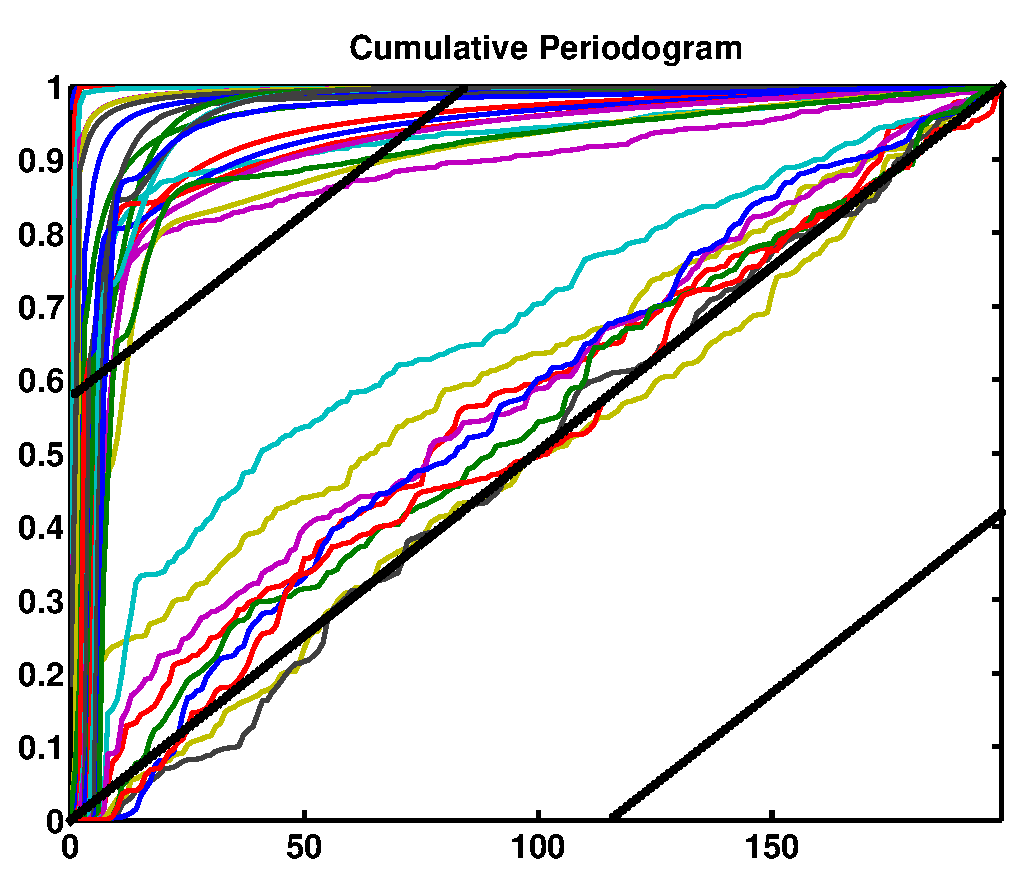
\includegraphics[width=.95\linewidth]{figures/run2/cum_per} 
   
	\end{minipage}
	\begin{minipage}[t]{0.5\textwidth}
	
		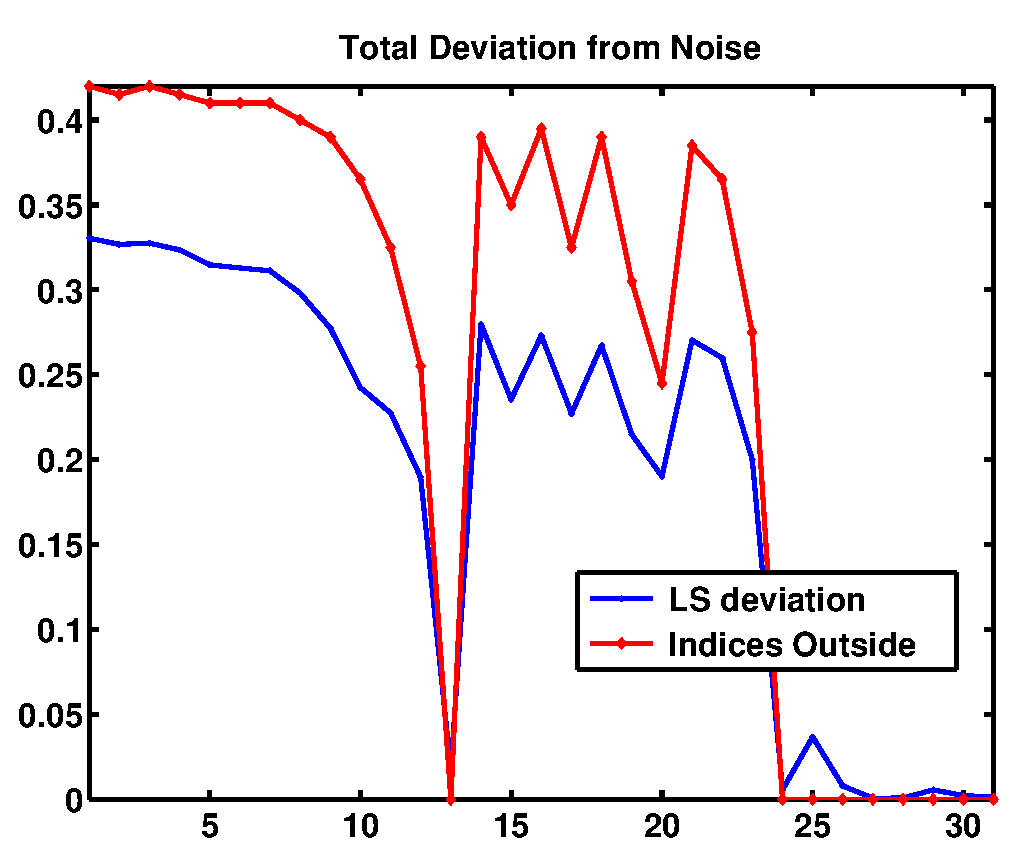
\includegraphics[width=.95\linewidth]{figures/run2/total_deviation} 
   
	\end{minipage}
	\vspace{5mm}
	{\centering $\delta_{noise}=10^{-8}$}
	%%%%%%%%%%%%%%%%%%%%%%%%%%%%%%%%%%%%%%%%%%%%%%
	
	%%%%%%%%%%%%%%%%%%%%%%%%%%%%%%%%%%%%%%%%%%%%%%
	\vspace{5mm}
	\begin{minipage}[t]{0.5\textwidth}
	
		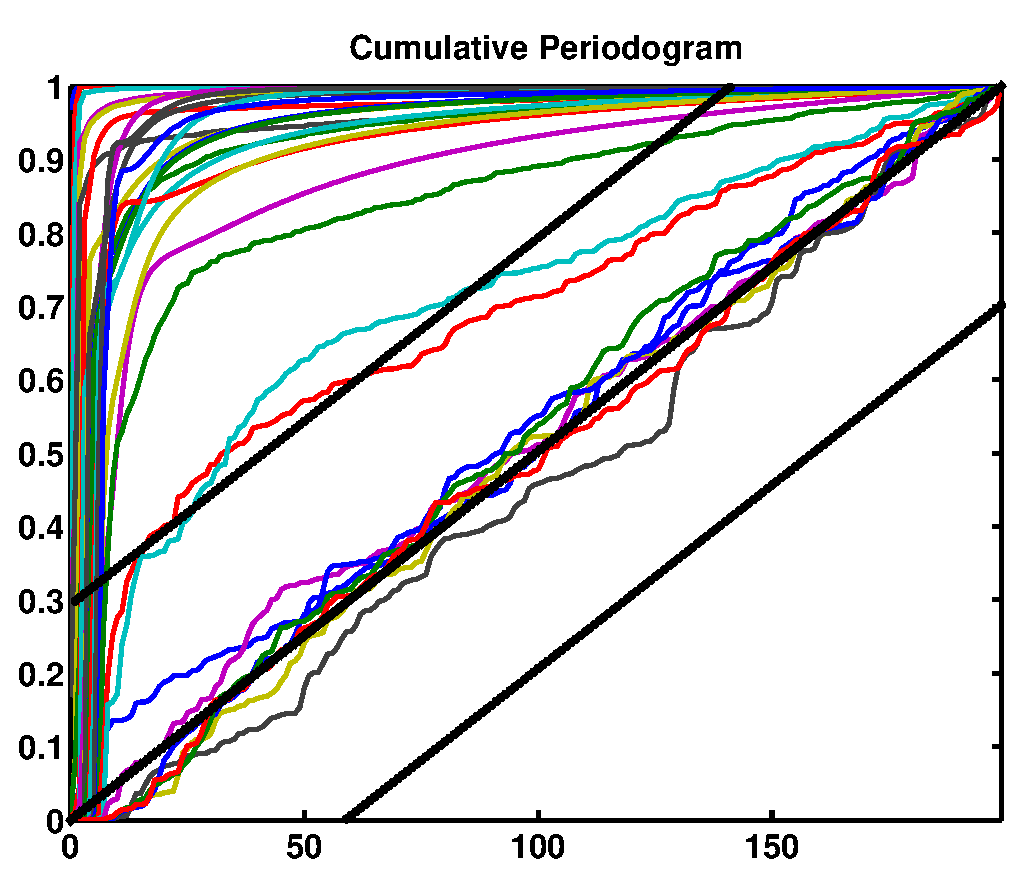
\includegraphics[width=.95\linewidth]{figures/run3/cum_per} 
   
	\end{minipage}
	\begin{minipage}[t]{0.5\textwidth}
	
		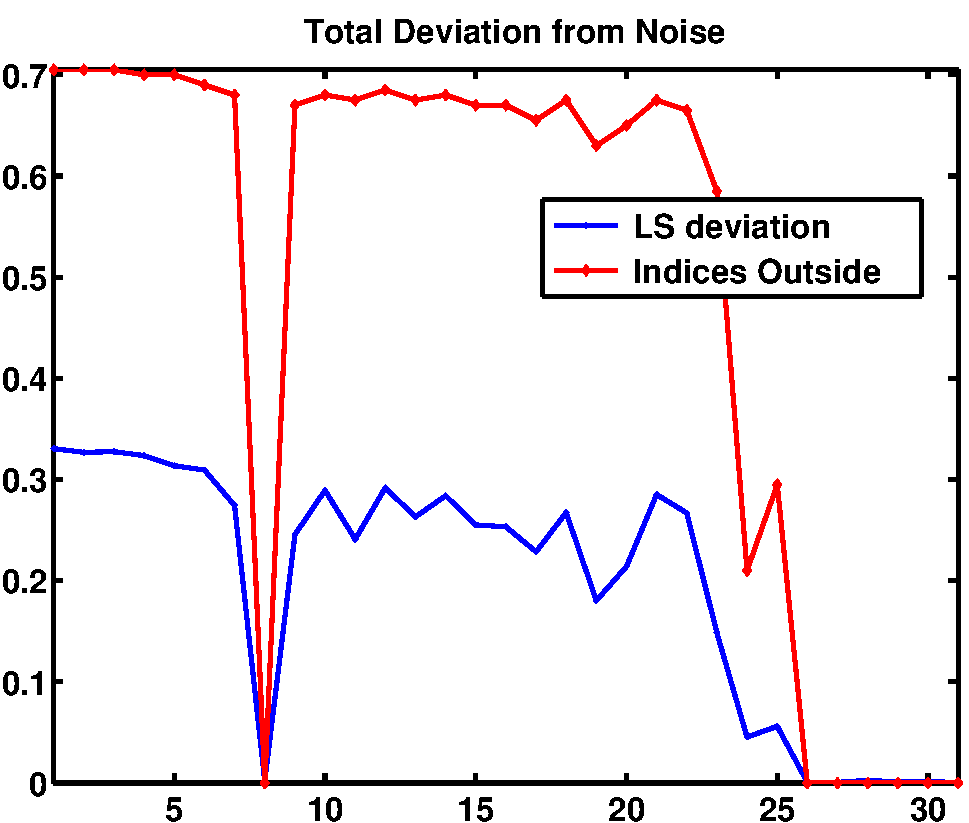
\includegraphics[width=.95\linewidth]{figures/run3/total_deviation} 
   
	\end{minipage}
	\vspace{5mm}
	{\centering $\delta_{noise}=10^{-4}$}
	%%%%%%%%%%%%%%%%%%%%%%%%%%%%%%%%%%%%%%%%%%%%%%
	
	%%%%%%%%%%%%%%%%%%%%%%%%%%%%%%%%%%%%%%%%%%%%%%
	\vspace{5mm}
	\begin{minipage}[t]{0.5\textwidth}
	
		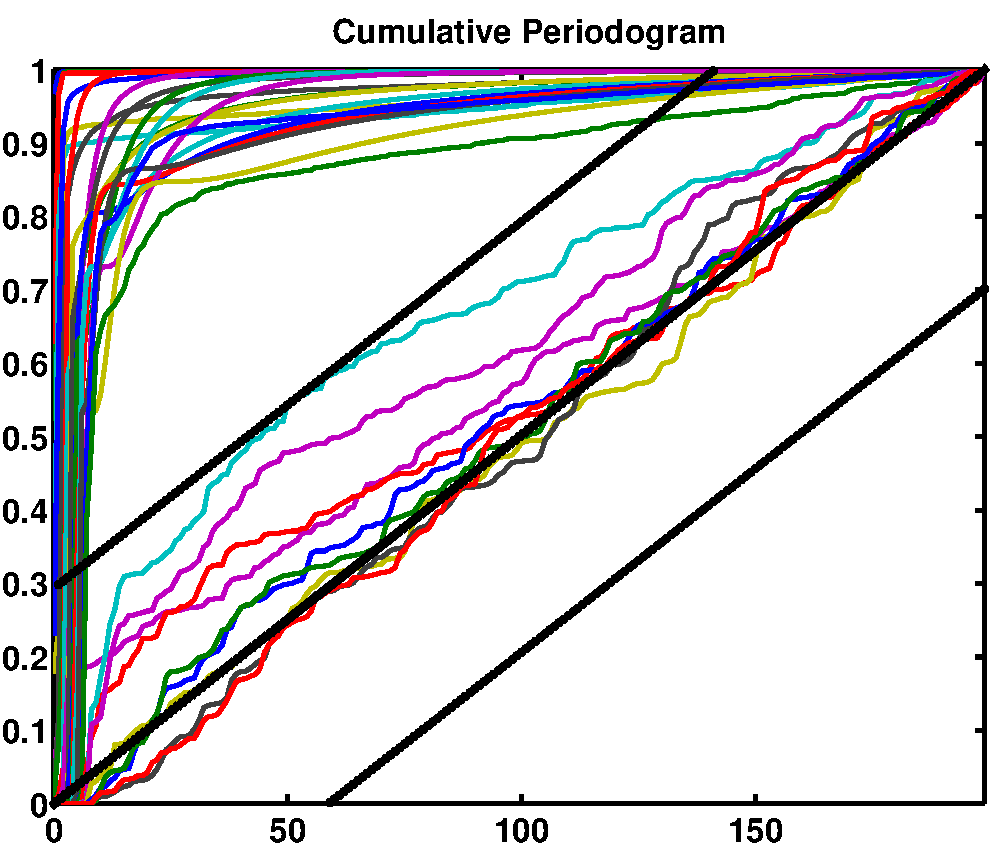
\includegraphics[width=.95\linewidth]{figures/run4/cum_per} 
   
	\end{minipage}
	\begin{minipage}[t]{0.5\textwidth}
	
		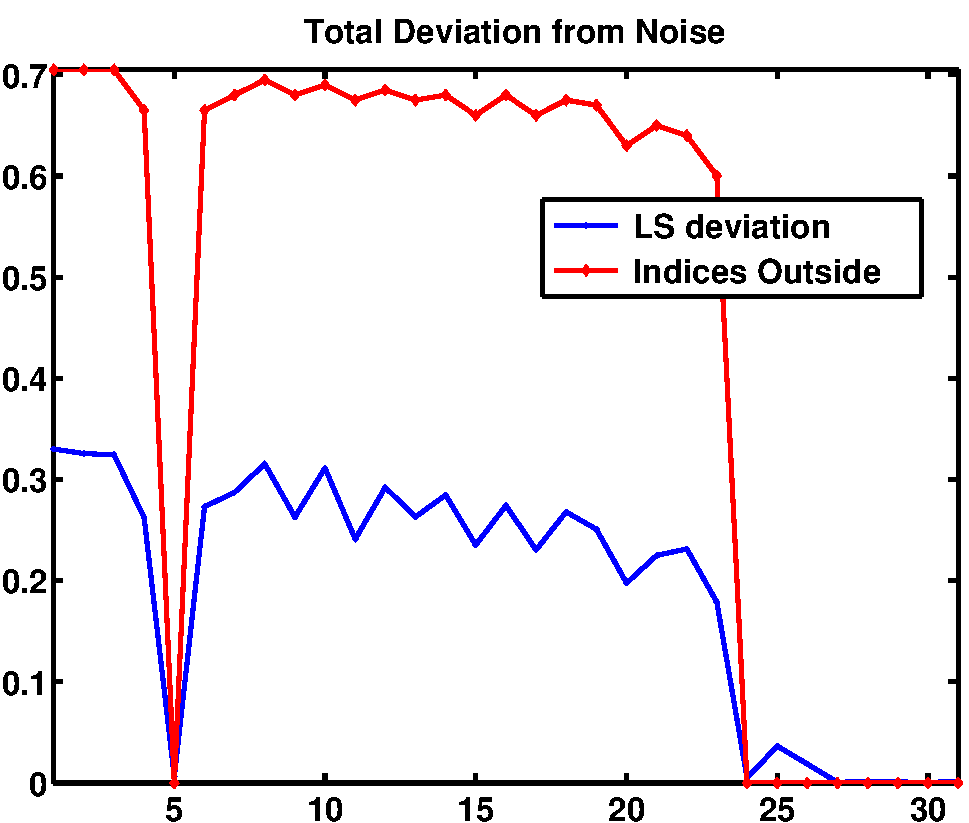
\includegraphics[width=.95\linewidth]{figures/run4/total_deviation} 
   
	\end{minipage}
		\vspace{5mm}
		{\centering $\delta_{noise}=10^{-2}$}
	%%%%%%%%%%%%%%%%%%%%%%%%%%%%%%%%%%%%%%%%%%%%%%


\begin{thebibliography}{1}
  \bibitem{bidiagonalization}  Hnetynkova, I. and Plesinger, M.. 
    \emph{The regularizing effect of the Golub-Kahan iterative bidiagonalization 
      and revealing the noise level in the data.}
      BIT Numer Math (2009) 49: 669-696.
    \bibitem{hansen} [17] Ivete
   \bibitem{svdRef} [10] Arthur will fill it in
\end{thebibliography}

\end{document}  
